\subsection{25 августа. Д.р. Кичкинекол}
\textit{Метеоусловия: утром, днём тепло, переменная обласность; после 17:00 дождь с грозой}

\begin{figure}[h!]
	\centering
	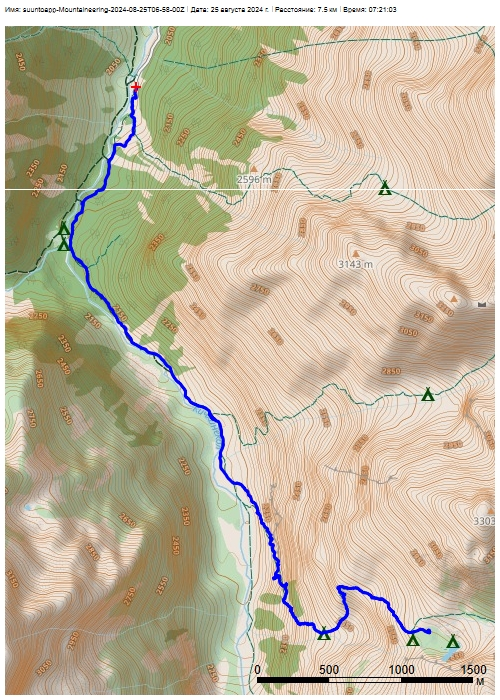
\includegraphics[angle=0, width=0.7\linewidth]{../pics/mini_maps/25}
	\label{fig:mini_25}
\end{figure}

Подъём в 6:30. Облачно, без осадков. Перепаковываемся (рис.~\ref{fig:DSC_0126.JPG}), оставляем некоторые вещи и продукты сходившему участнику группы (Наташе). 

\begin{figure}[h!]
	\centering
	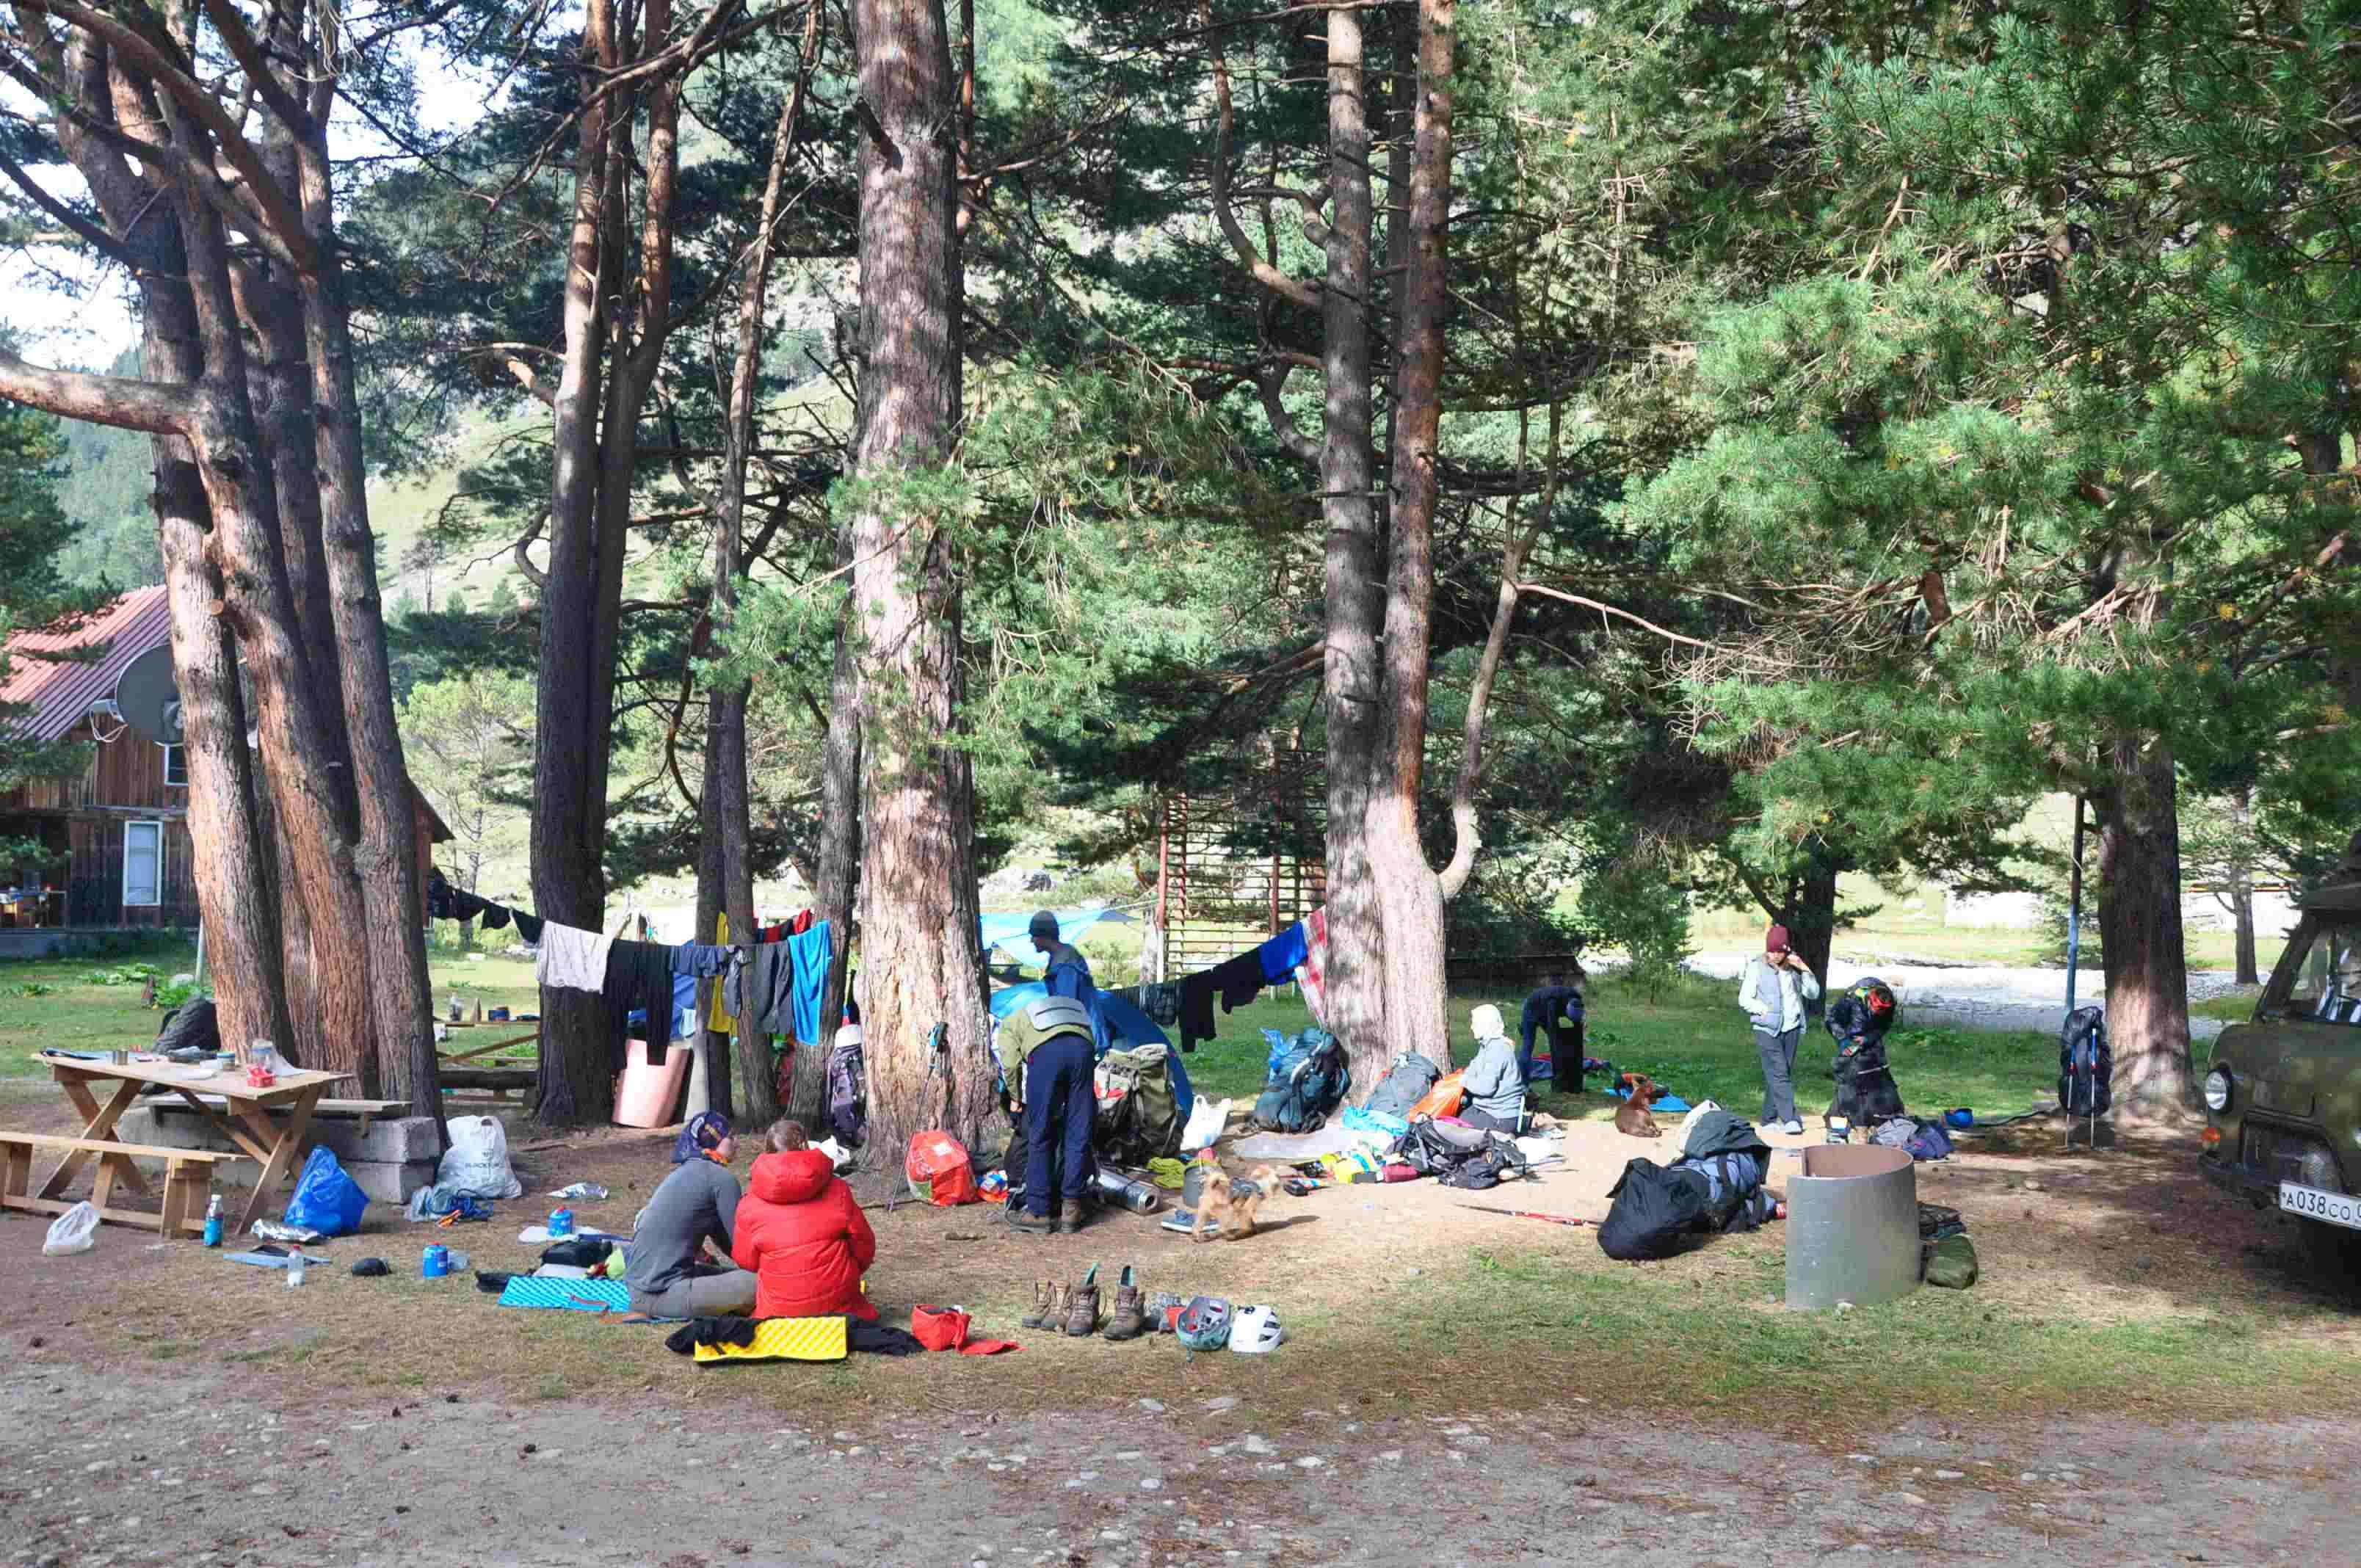
\includegraphics[width=0.7\linewidth]{../pics/DSC_0126.JPG}
	\caption{Утренние сборы в а/л <<Узункол>>}
	\label{fig:DSC_0126.JPG}
\end{figure}

Выходим в 9:58 по левому берегу р. Узункол. В 10:45 оказываемся в ущелье р. Кичкинекол (рис.~\ref{fig:DSC_0127.JPG}). 

\begin{figure}[h!]
	\centering
	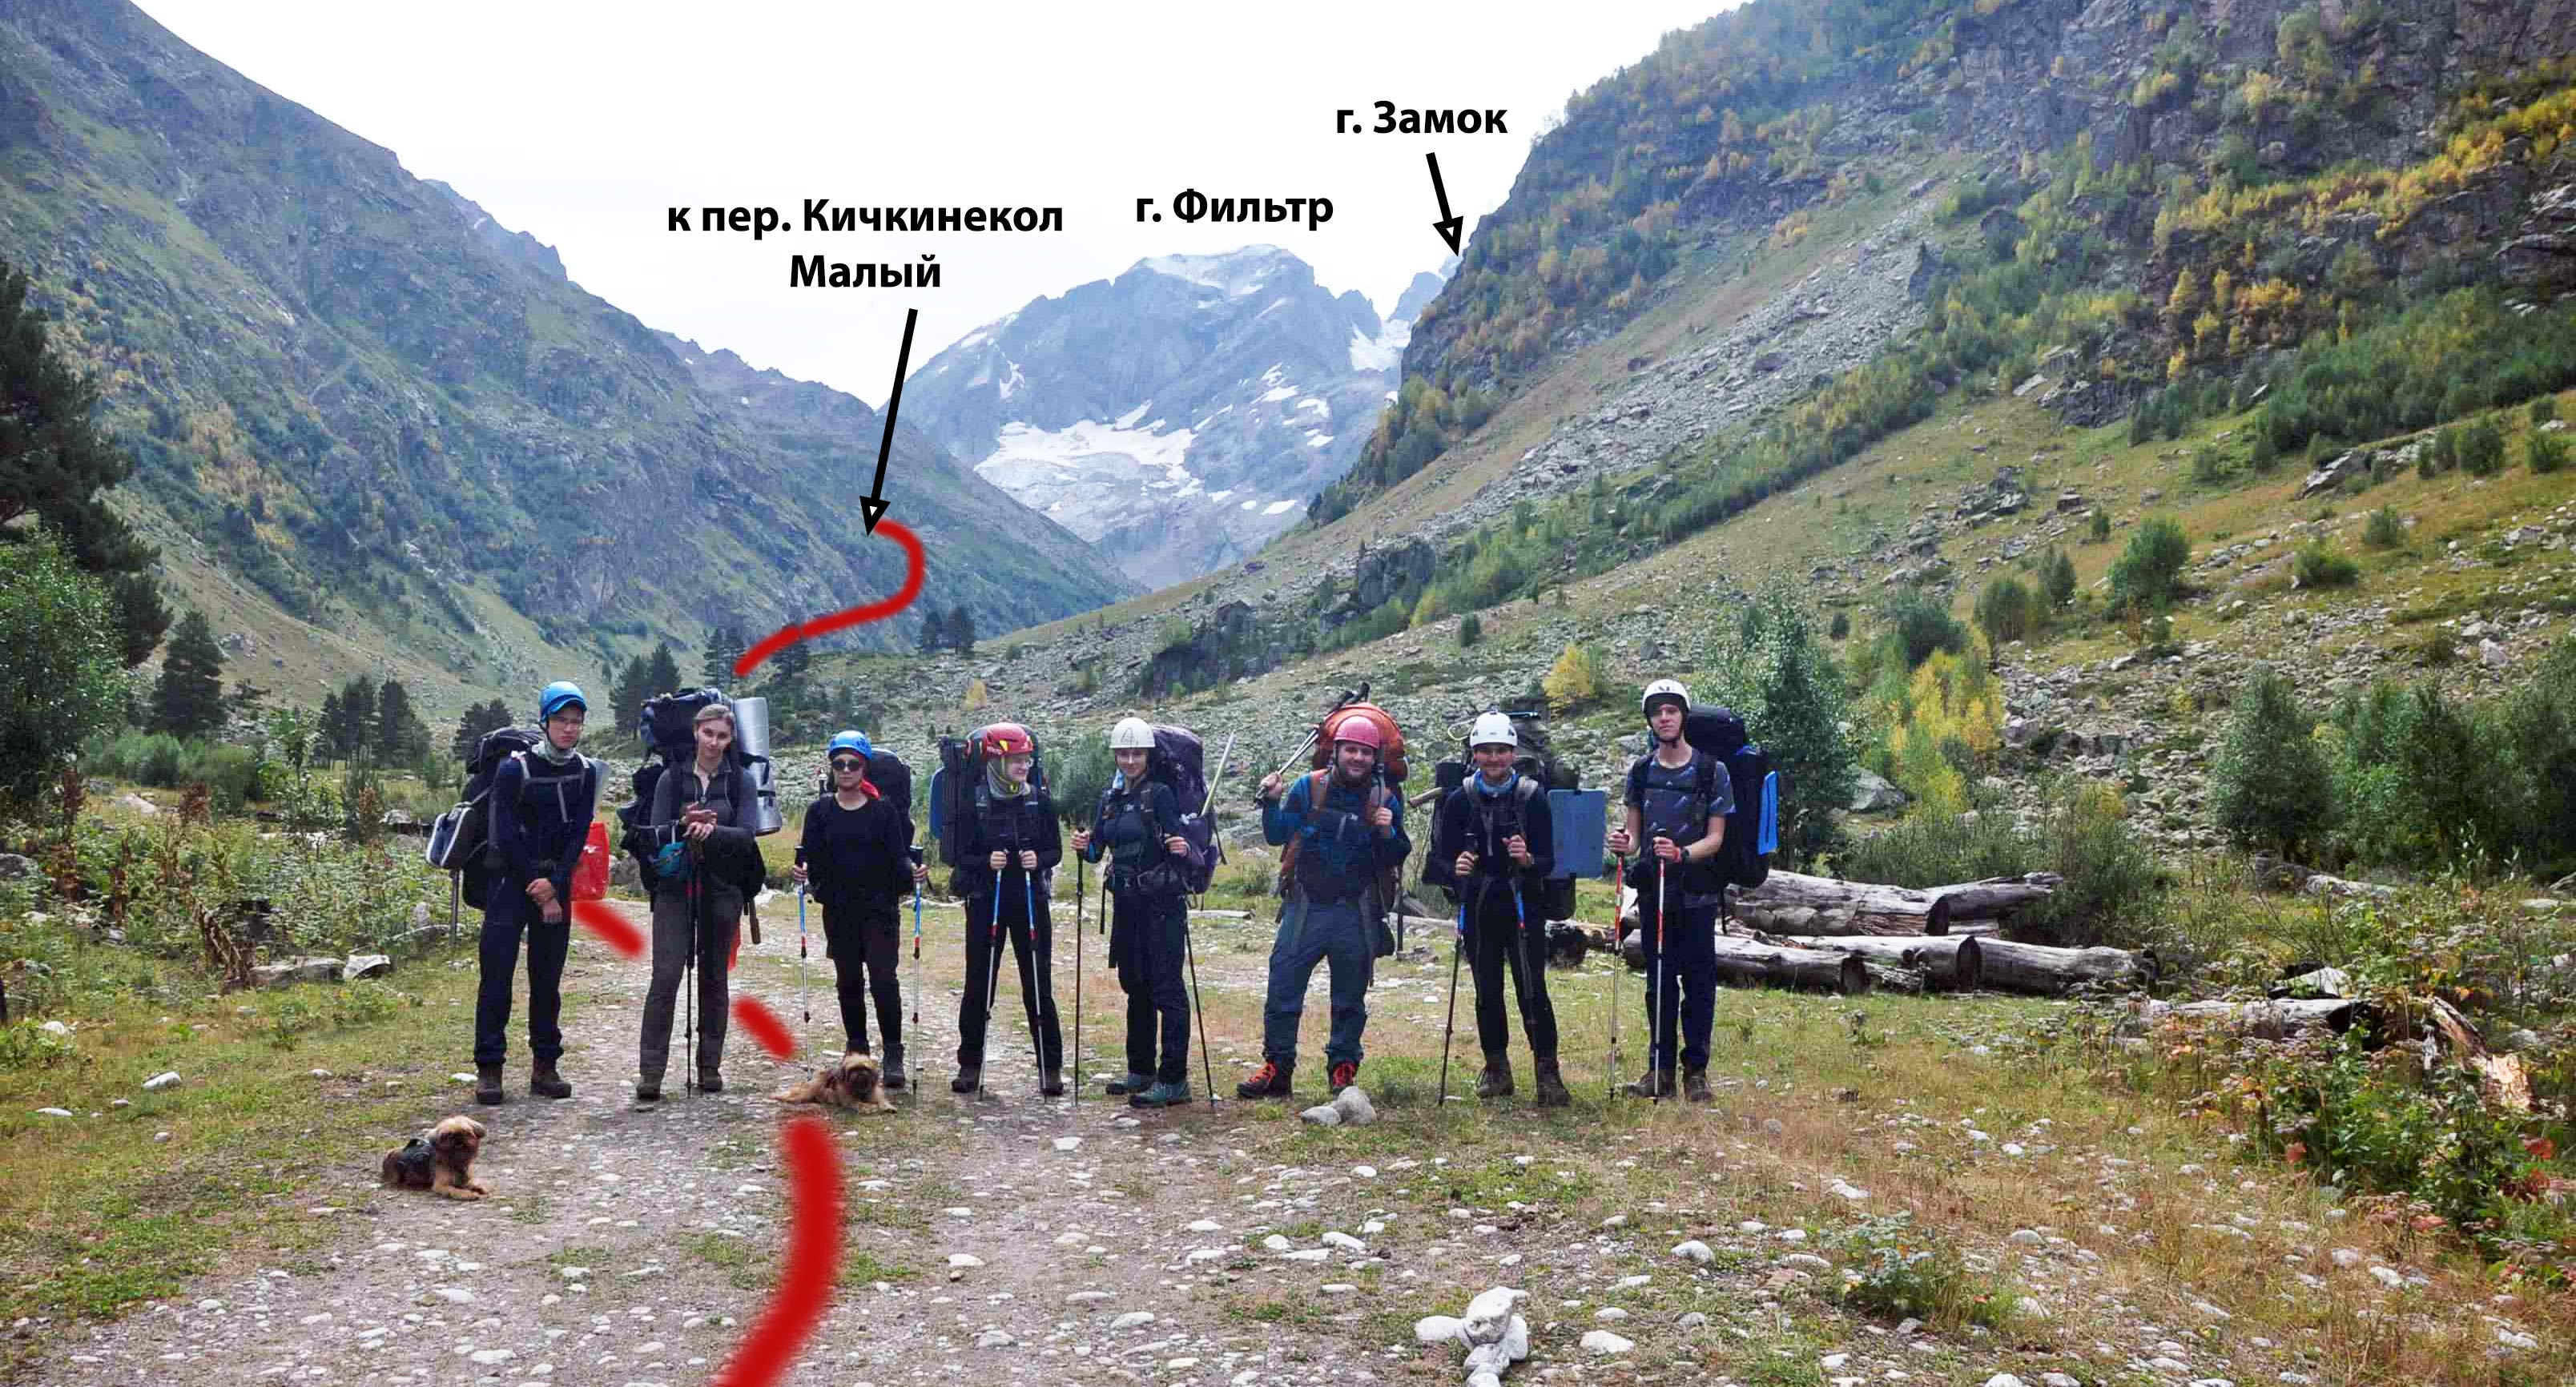
\includegraphics[width=0.7\linewidth]{../pics/DSC_0127.jpg}
	\caption{группа в ущелье р. Кичкинекол}
	\label{fig:DSC_0127.JPG}
\end{figure}


Грунтовка укатанная, регулярно проезжают машины.  В 11:12 проходим поворот на пер. Доломиты Южные (1А). Боясь пропустить поворот на косогор, ведущий к нашему перевалу Кичкинекол Малый, забираемся на склон, как оказывается позднее, за 200 м до начала тропы, и в 11:50 подсекаем хорошо набирую тропу (рис~\ref{fig:IMG_20240825_134744.jpg}).  
	
	\begin{figure}[h!]
		\centering
		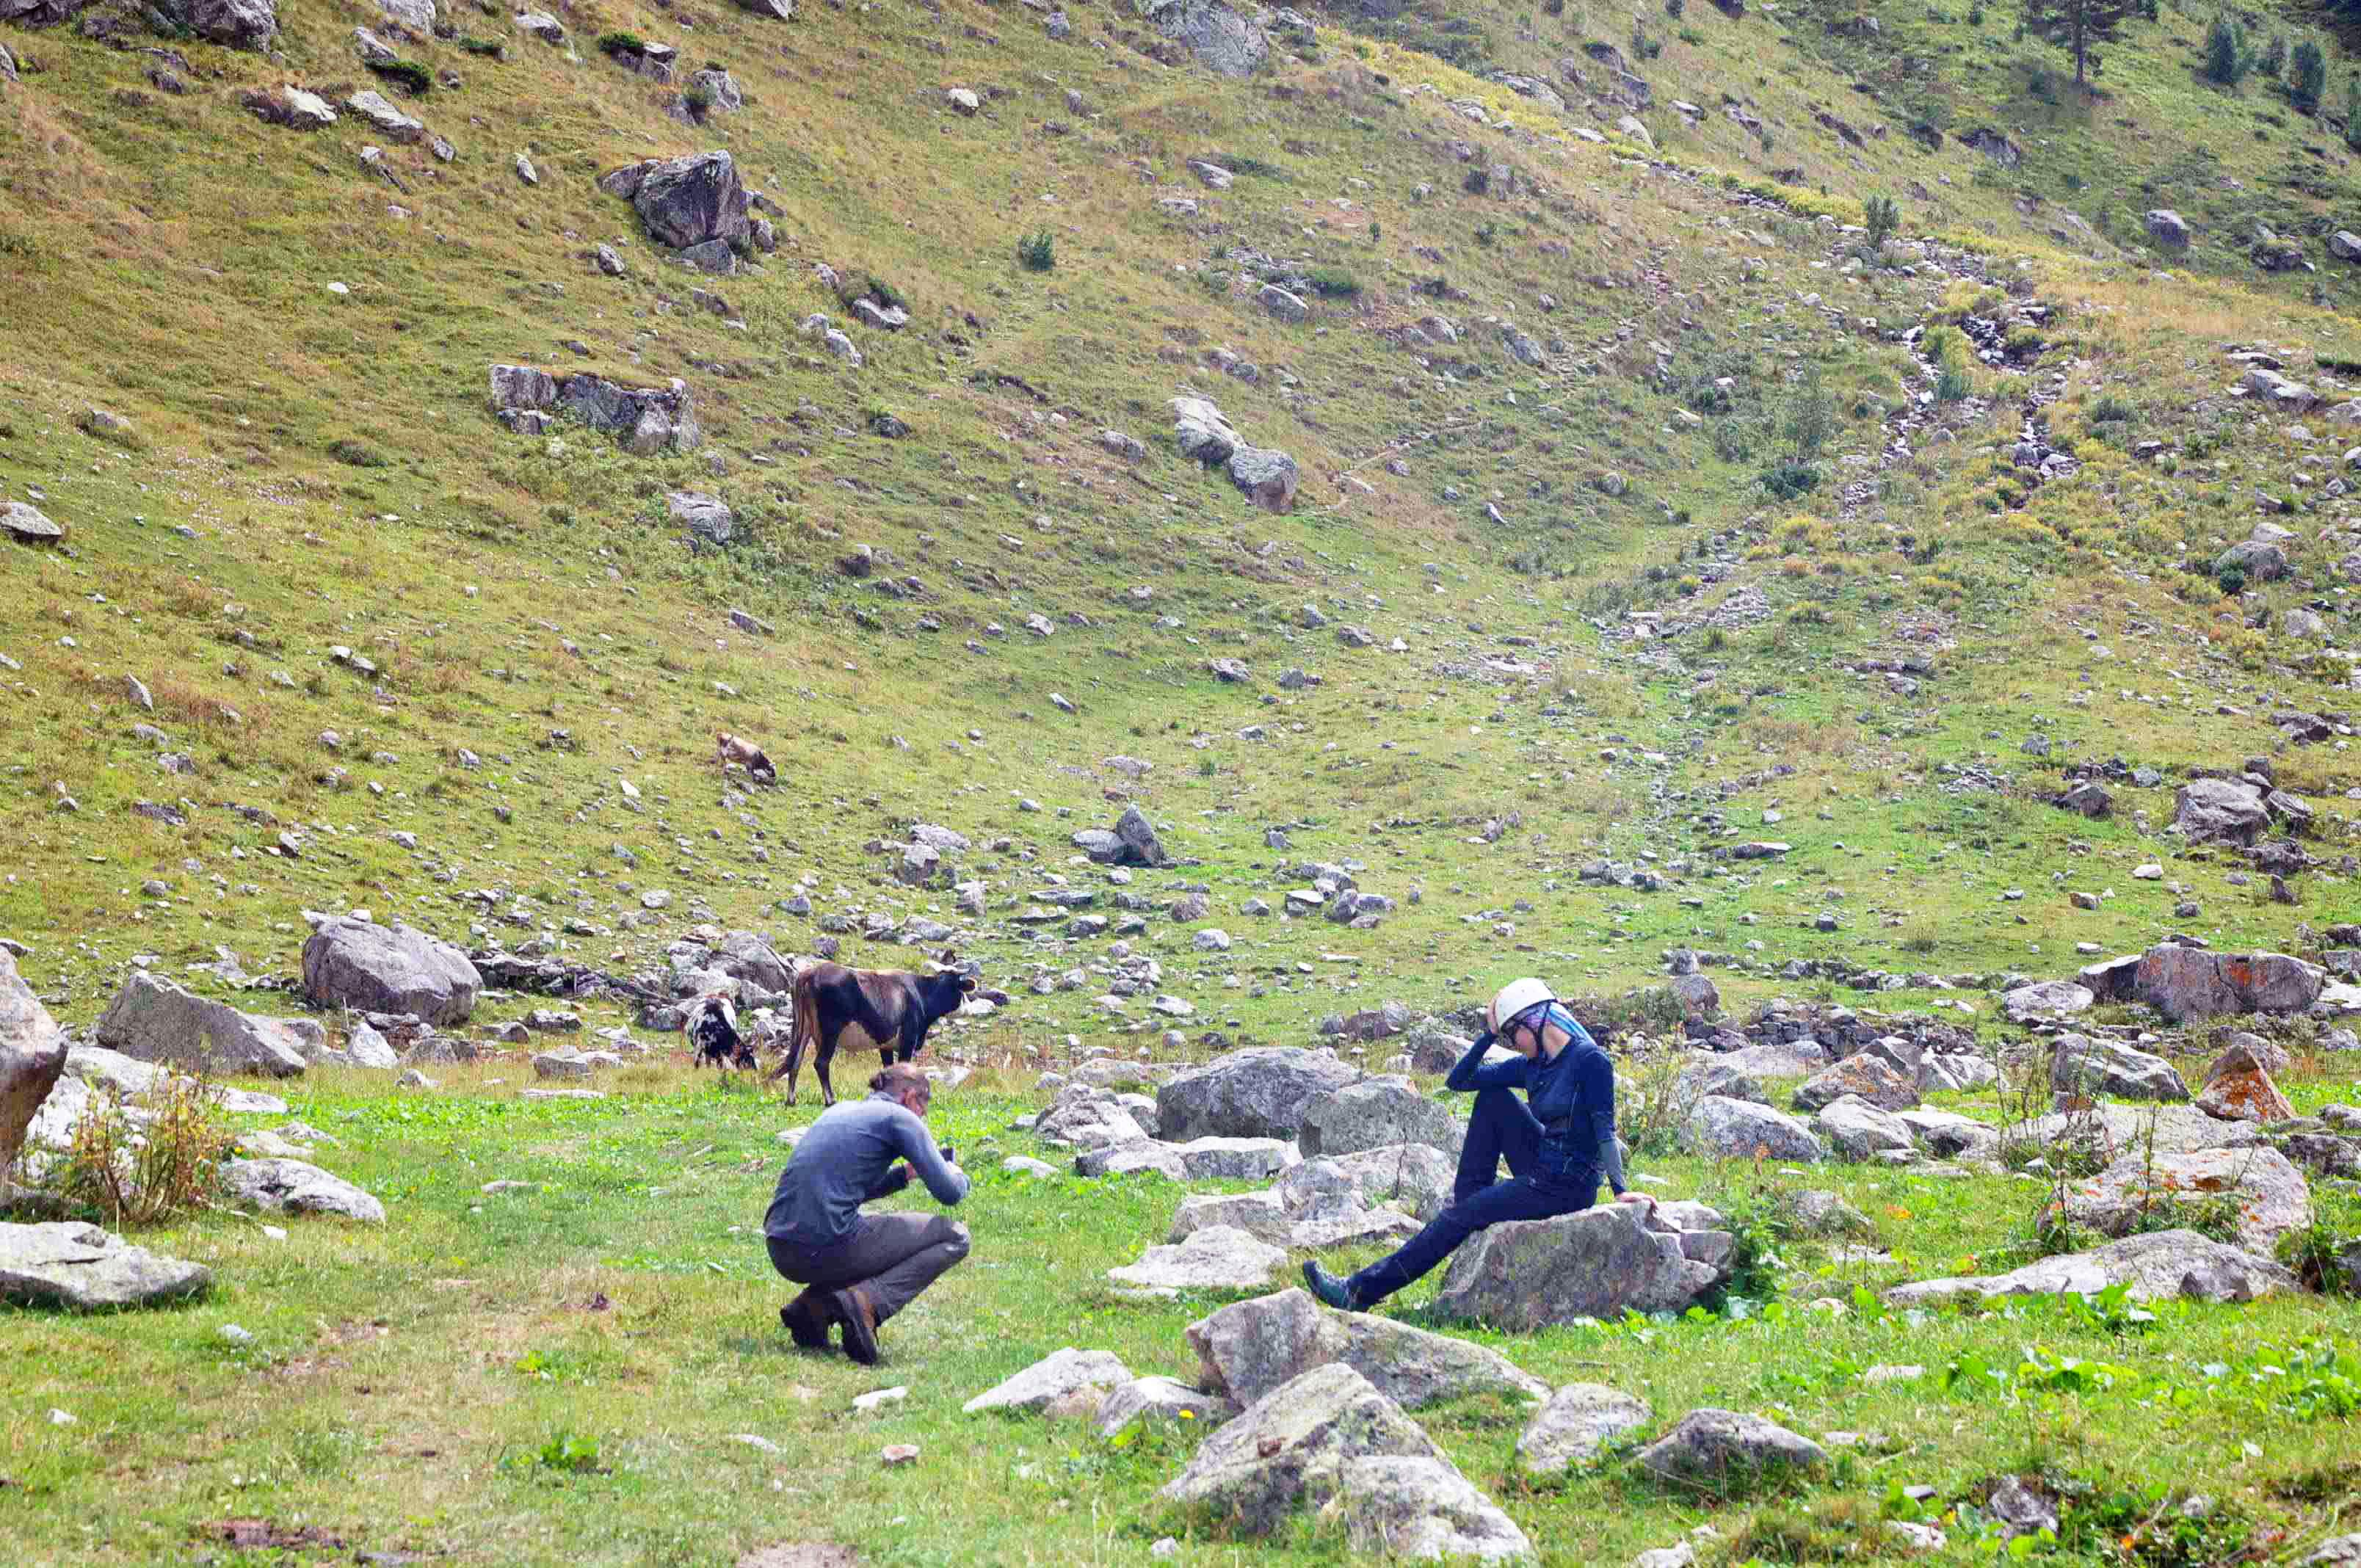
\includegraphics[width=0.7\linewidth]{../pics/DSC_0138.jpg}
		\caption{Начало подъёма на косогор в д.р. Таллычат}
		\label{fig:DSC_0138.JPG}
	\end{figure}
	
	Возле водопада, на высоте 2365~м, в 13:06 делаем привал, чтобы набрать воды и поискать потерянные на переходе блокнот и бинокль (к сожалению, безуспешно). Далее по тропе набираем высоту по графику 15/10 минут. Погода была всё ещё пасмурной, но ничего движению не мешало. Мест для обеда не было, поэтому питались заначкой и сух.пайком.

\begin{figure}[h!]
	\centering
	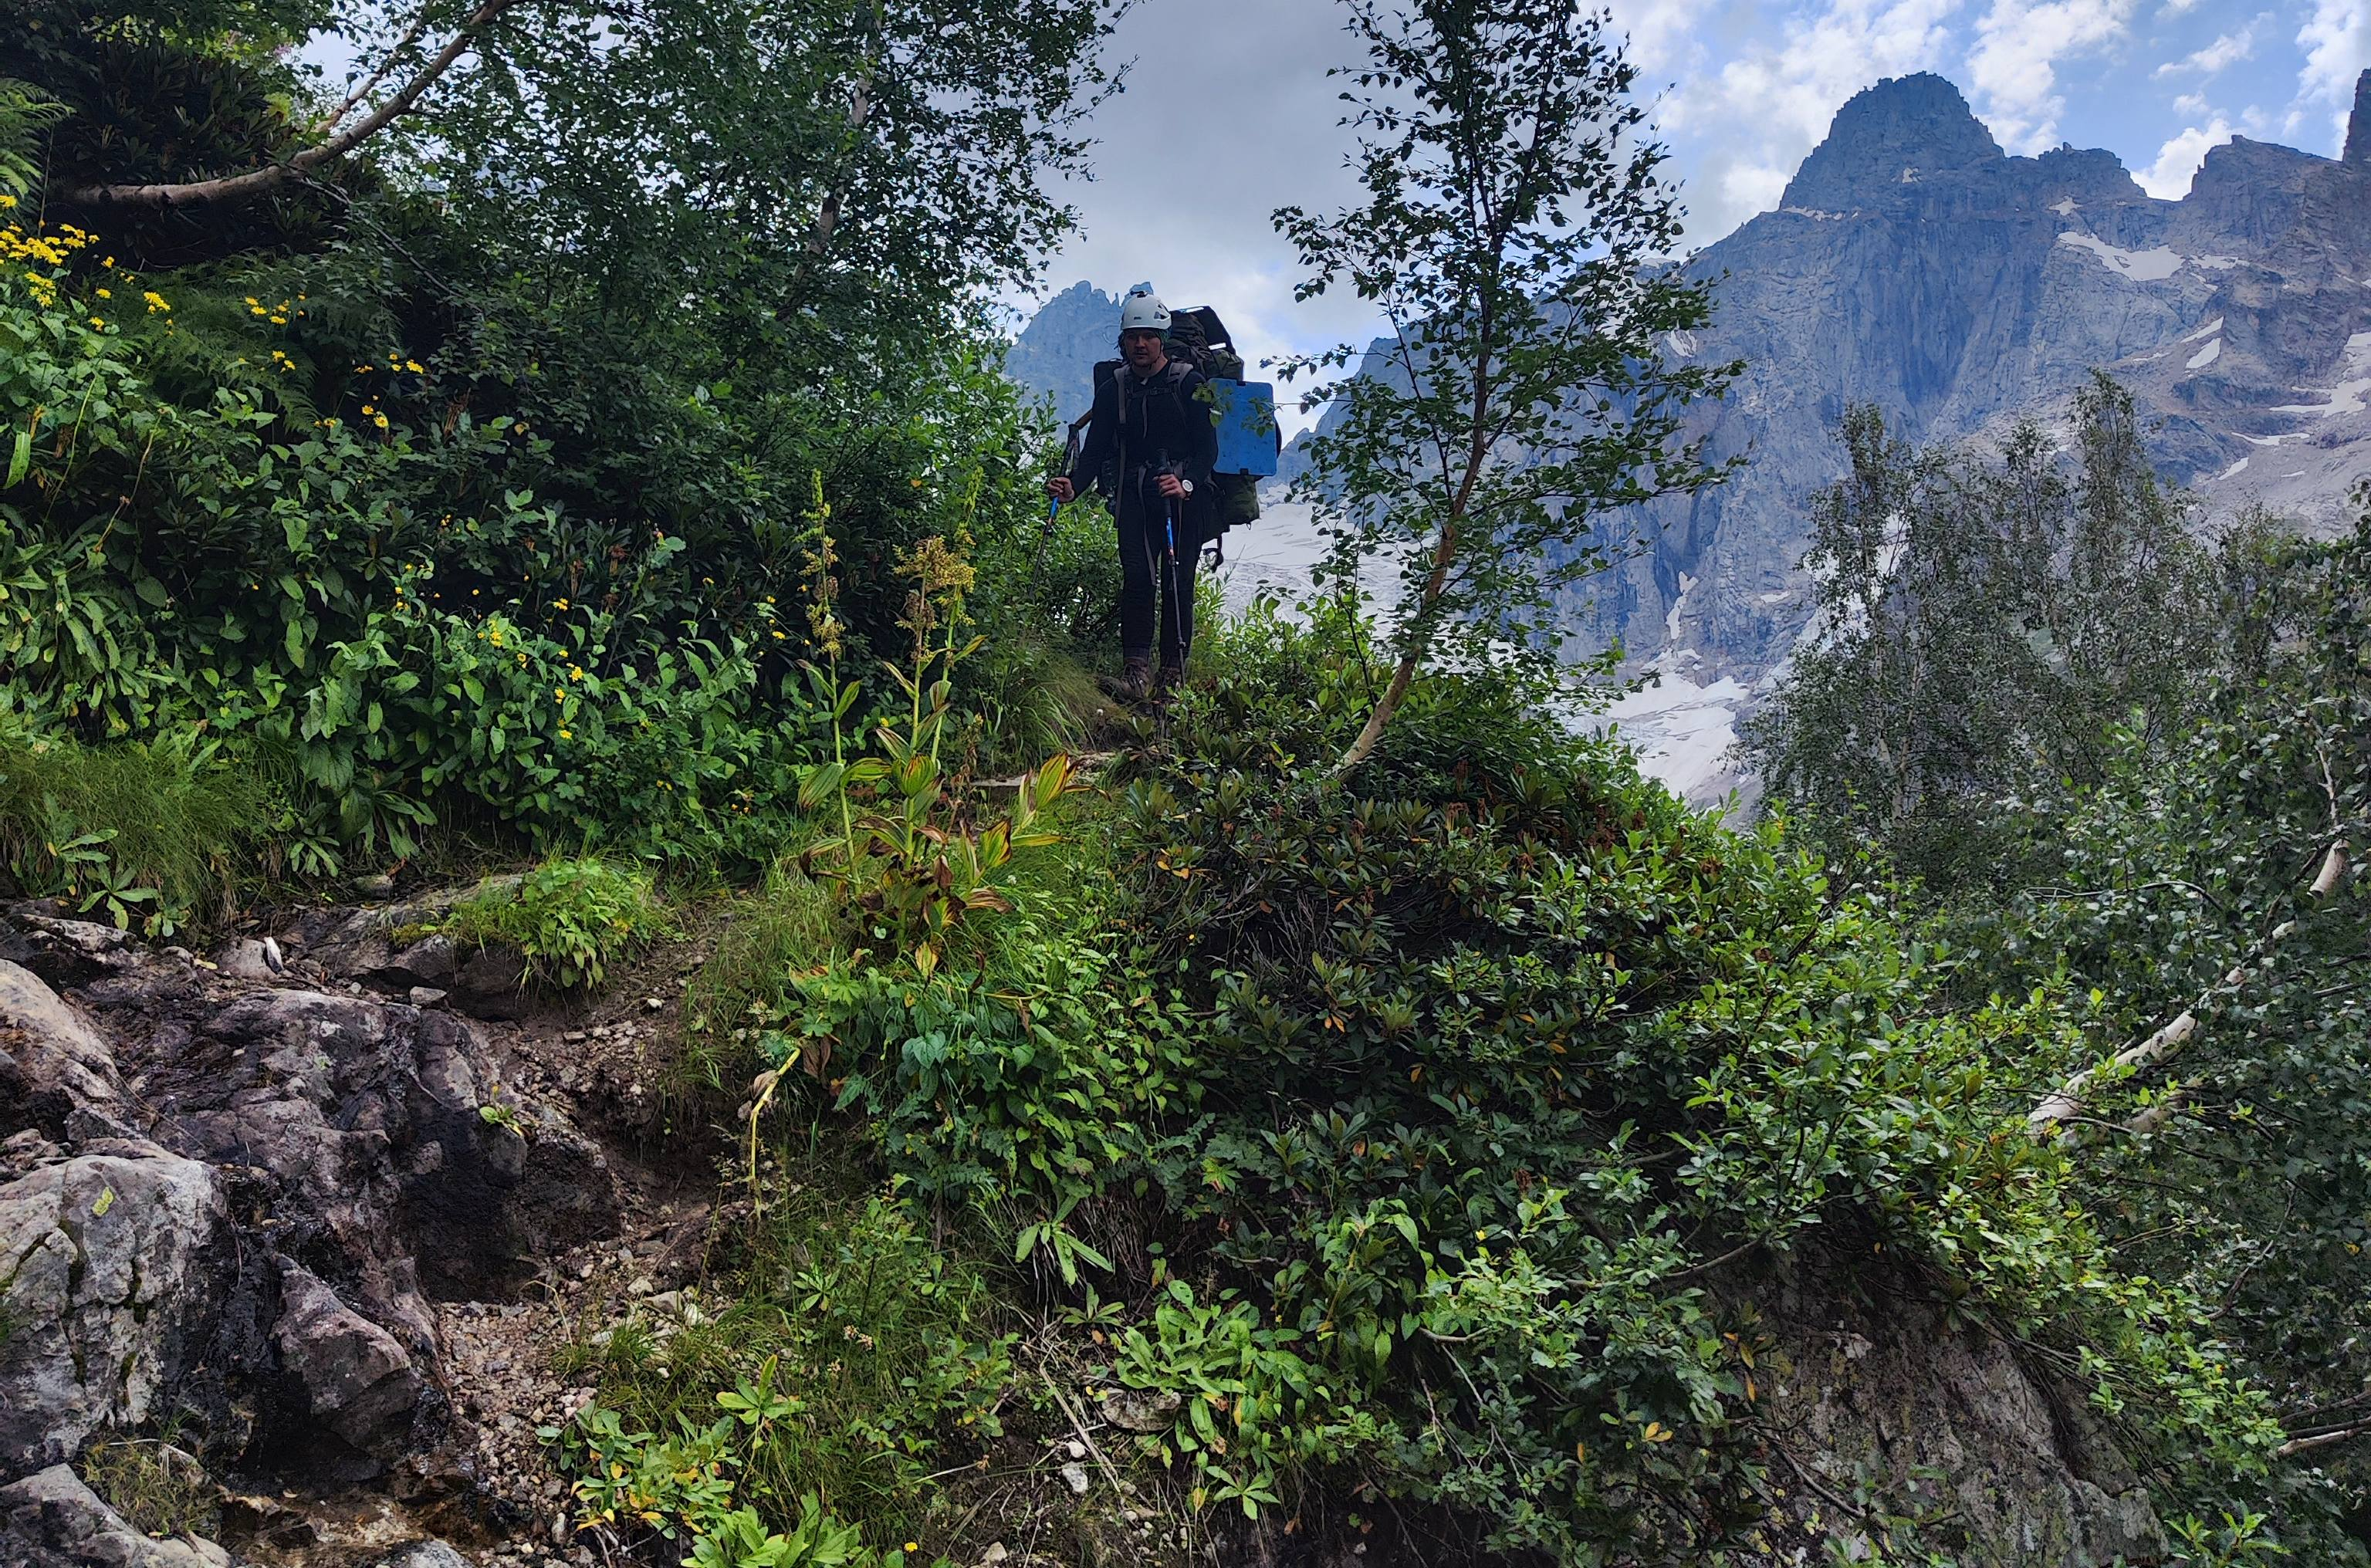
\includegraphics[width=0.7\linewidth]{../pics/IMG_20240825_134744.jpg}
	\caption{Тропа по склону р. Кичкинекол к Таллычатским ночёвкам}
	\label{fig:IMG_20240825_134744.jpg}
\end{figure}


В 14:40 выходим из зоны леса к нижним Таллычатским ночёвкам. Нашему взору представляются потрясающие виды на ГКХ (рис.~\ref{fig:DSC_0158.JPG}). 

\begin{figure}[h!]
	\centering
	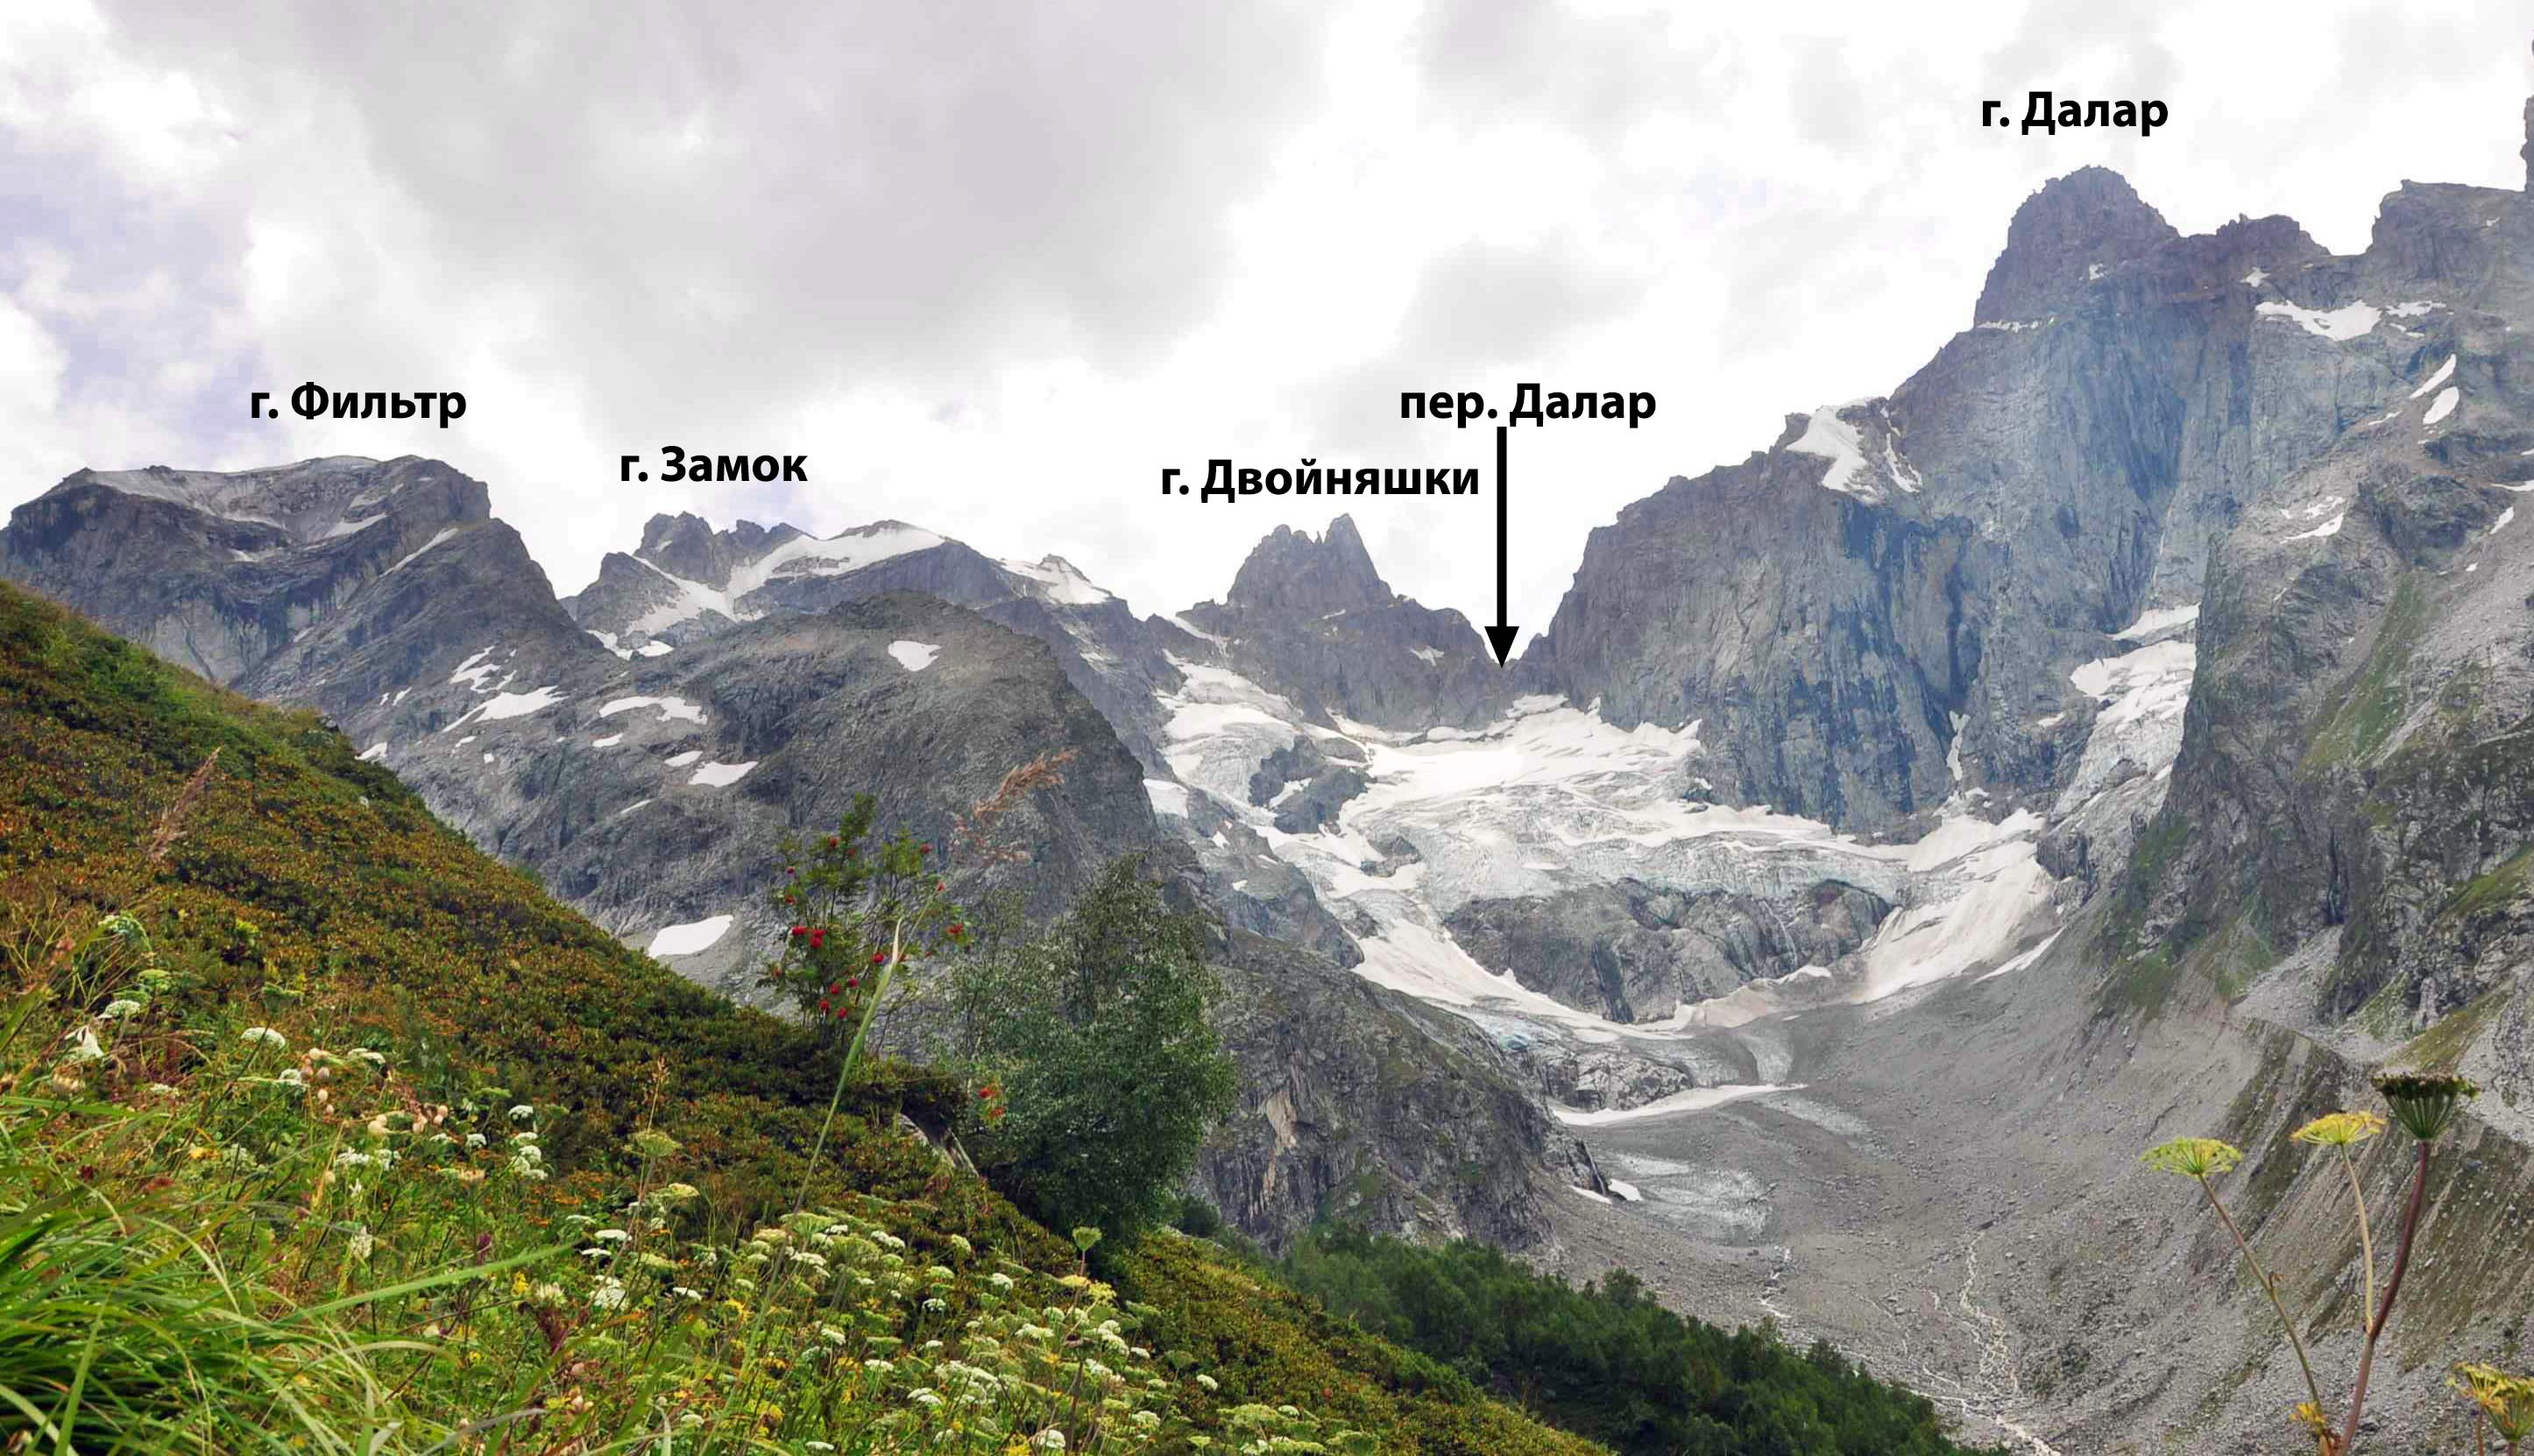
\includegraphics[width=0.7\linewidth]{../pics/DSC_0158.jpg}
	\caption{Вершины и перевалы ГКХ в районе пер. Кичкинекол}
	\label{fig:DSC_0158.JPG}
\end{figure}

Дальшейший путь до м.н. не представляет особого труда, если не учитывать красивые виды вокруг и обилие костяники под ногами.

В 16:04 приходим на наше м.н., пересохшее озеро, называющееся сейчас Поляной Крокусов. Ставим палатки, готовим ужин, и сразу после этого начинается сильный дождь. Непогода не прекращалась до часу ночи, некоторые участники были вынуждены рыть дренажные канавы, чтобы не затапливало палатки. Утром мы порадовались, что встали в верхней части стоянок, так как нижняя часть озера за ночь перестала быть пересохшей.
Координаты м.н. N43.249638\degree, E42.198292\degree.

\begin{figure}[h!]
	\centering
	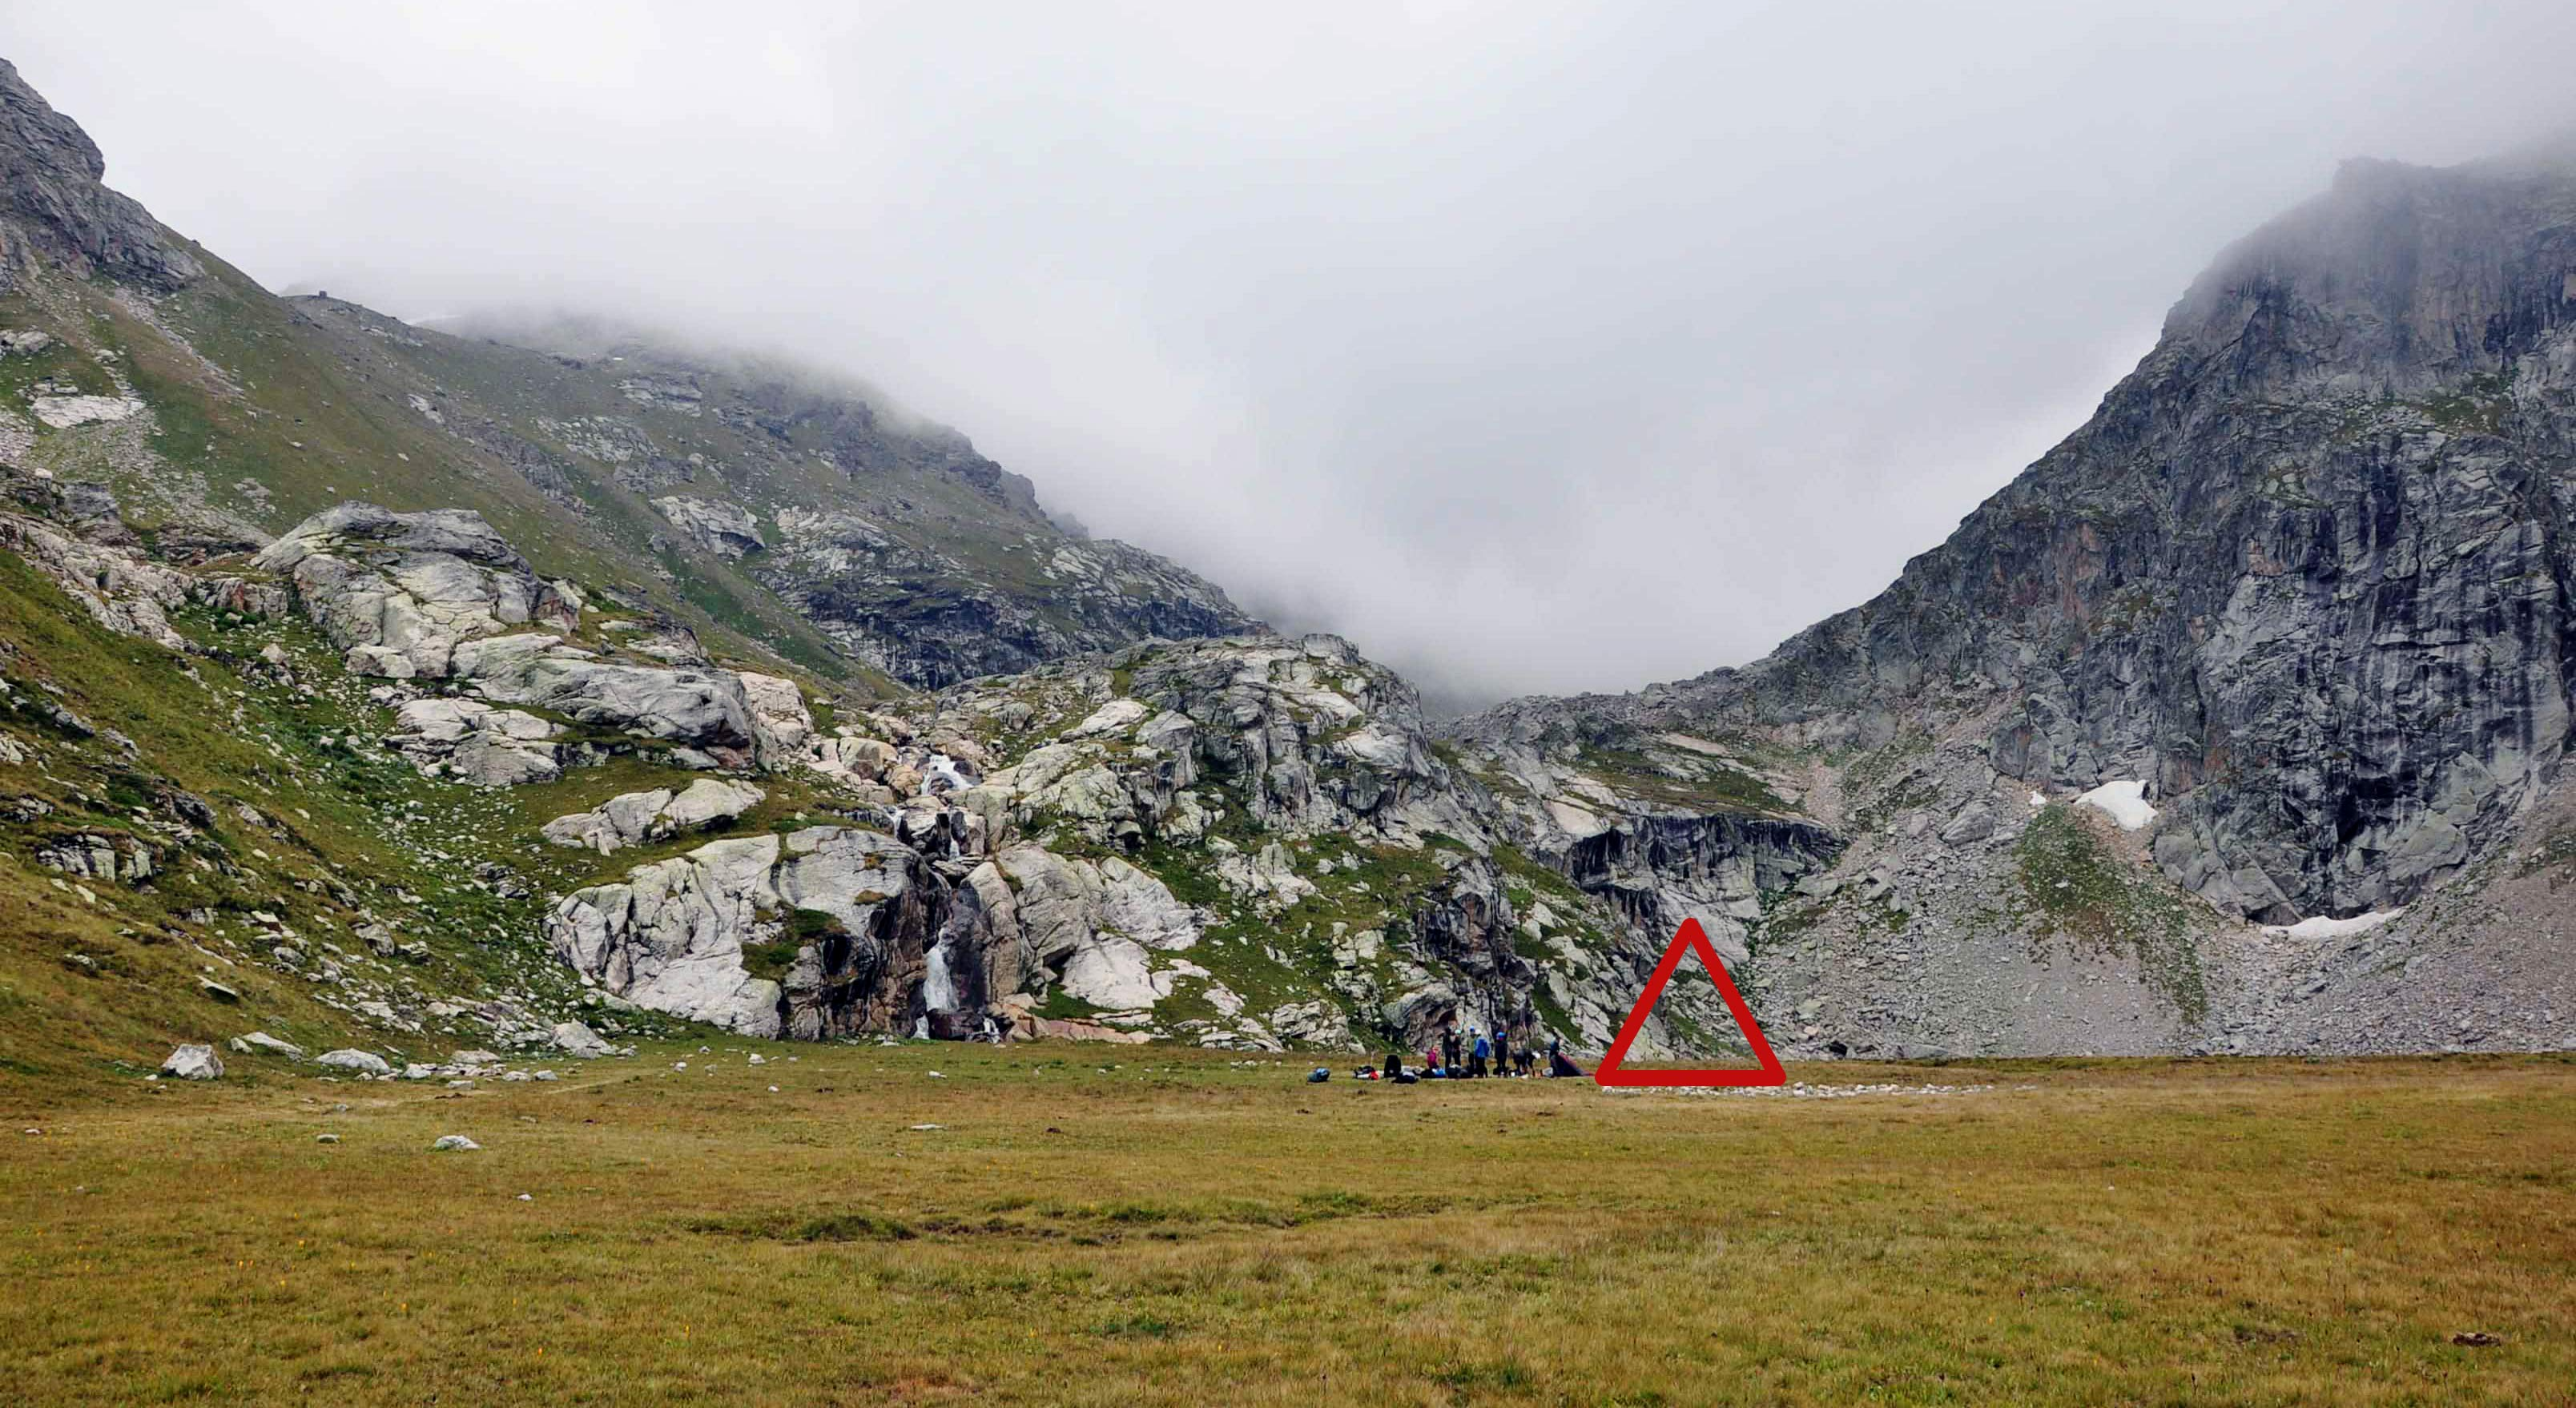
\includegraphics[width=0.7\linewidth]{../pics/DSC_0177.jpg}
	\caption{м.н. 25-26 августа}
	\label{fig:DSC_0177.JPG}
\end{figure}




\newpage